\section{\textcolor[HTML]{D32F2F}{Forarbeid}}

%domenekunnskap
Når man jobber med brukersentrert design er det nettopp brukeren som skal være i sentrum. Beslutninger skal tas med brukeren i tankene, og ingen ting skal overlates til tilfeldighetene. Gruppen fulgte derfor seks prinsipper for brukersentrert design:
\begin{enumerate}
    \item Designet skal være basert på̊ en eksplisitt forstå̊else av brukerne, deres oppgaver og omgivelser
    \item Brukere skal være involvert i hele design- og utviklingsprosessen
    \item Designet er drevet av brukersentrert evaluering
    \item Prosessen er iterativ
    \item Designet adresserer hele brukeropplevelsen
    \item Designteamet består av multidisiplinære perspektiv
\end{enumerate}

\noindent Ved å ha disse seks punktene i fokus sørget gruppen for at brukeren ble holdt i fokus gjennom hele prosessen. I tillegg til de seks punktene kan man også klassifisere brukersentrerte aktiviteter i fire kategorier. Disse kategoriene er: forståelse og spesifikasjon av brukskontekst; spesifikasjon av brukernes krav; produksjon av designløsninger som møter brukerkravene; og evaluering av design. Disse fire kommer i tillegg til planlegging og implementering.
\\\\
For å være sikker på at gruppen hadde forstått målgruppen til Sirkus shopping valgte gruppen å ta kontakt med senterlederen Cecilie Løseth. Gruppen hadde ikke noen intensjon om å skape personas etter målgruppen til senteret, men det var oppklarende å få svar på noen av spørsmålene som gruppen hadde. Senterlederen kunne fortelle at målgruppen for senteret er familier, personer 0-45 år i familiesituasjon og studenter.

\subsection{Lignende apper}
\label{lignendeApper}
For å få inspirasjon til å forbedre handleopplevelsen på Sirkus shopping utforsket gruppen to handleapplikasjoner. Gruppen valgt å se på \textit{Boozt} og \textit{Zalando}. Grunnen til at gruppen valgte å søke inspirasjon hos nettbutikker var fordi gruppen likte fleksibilitet nettbutikkene gir og ønsket å lage en applikasjon som kunne bli en mellomting mellom nettbutikk og butikk. Butikkene skal kunne være konkurransedyktige med nettbutikkene, med mulighet for en kunde å hente varer med en gang etter kjøp.

\subsubsection{Boozt}
Det gruppen likte med Boozt var struktureringen av elementer i handlekurv (til venstre i Figur \ref{fig:Boozt}) og oppsett av favoritter (midt i Figur \ref{fig:Boozt}). I tillegg til dette var symbolene øverst til høyre i Figur \ref{fig:Boozt} viktige for gruppen å bruke i en app da slike symboler er gjenkjennelige og knyttes opp mot designprinsippet om \textit{affordance}. 

\begin{figure}[H]
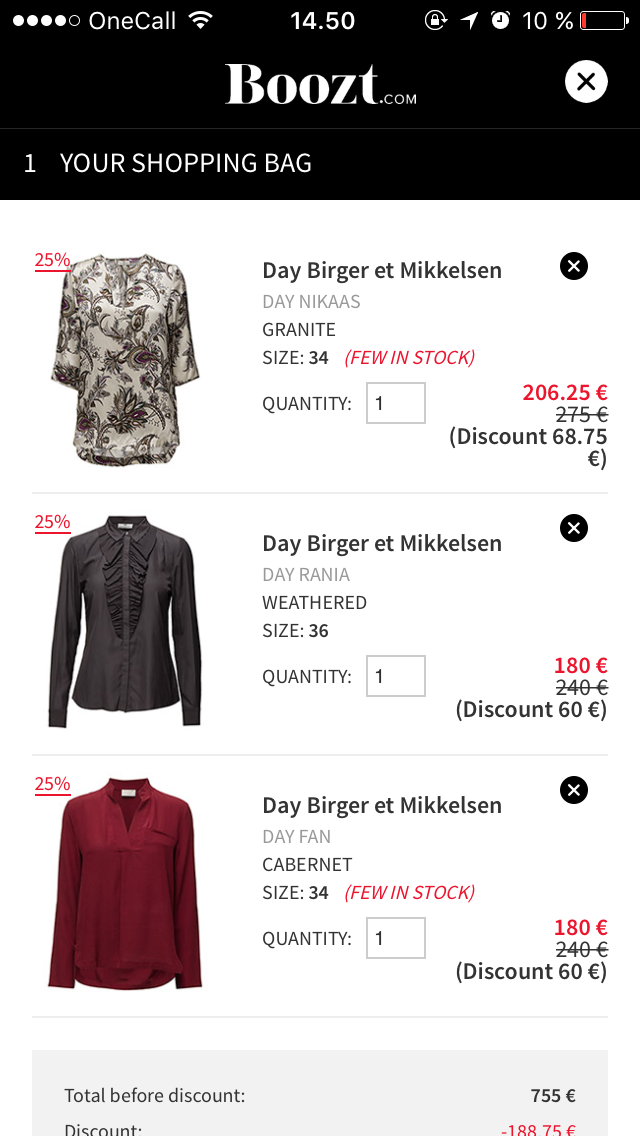
\includegraphics[scale=0.2]{images/inspiration/image1}
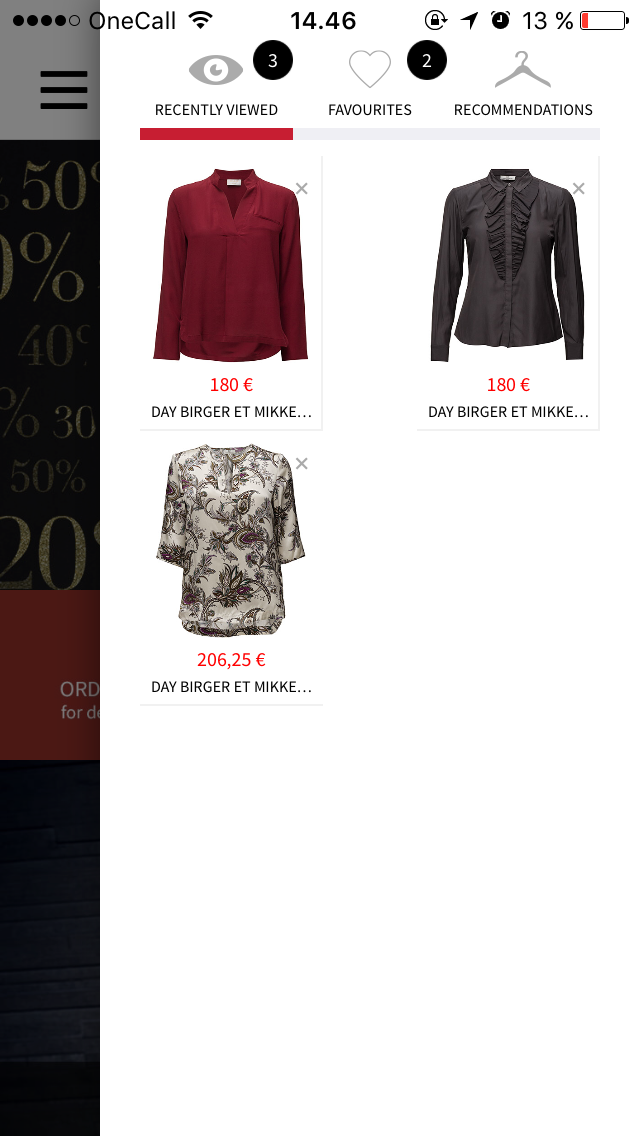
\includegraphics[scale=0.2]{images/inspiration/image2}
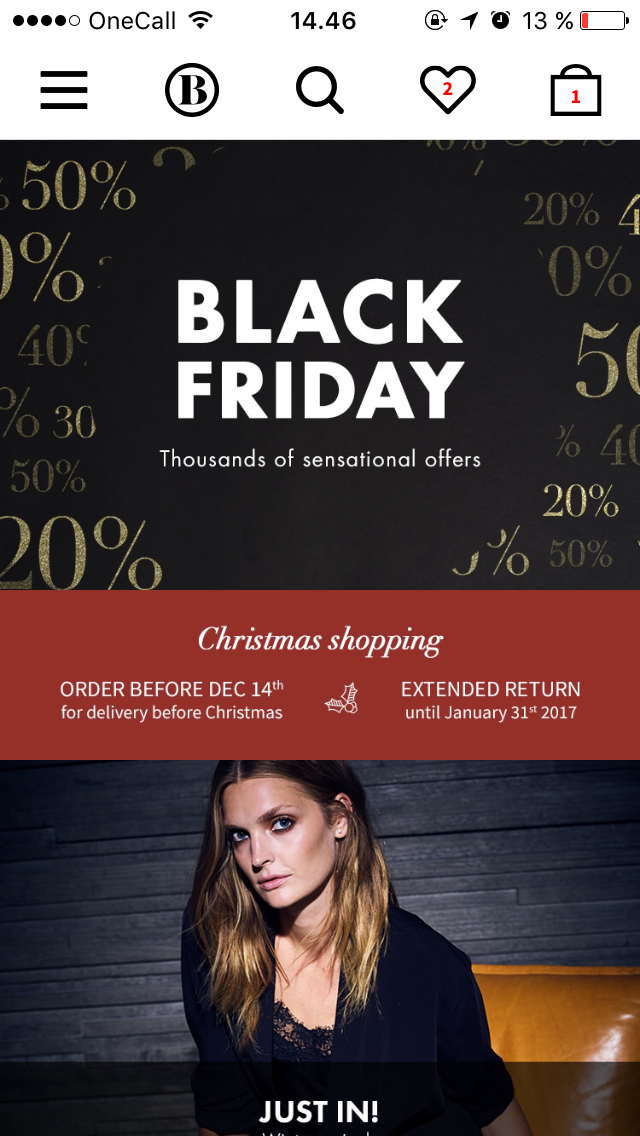
\includegraphics[scale=0.2]{images/inspiration/image3}
\centering %centering the image
\caption{Boozt}
\label{fig:Boozt}
\end{figure}

\subsubsection{Zalando}
\label{zalando}
Det gruppen likte med Zalando sin applikasjon var menylinjen med elementer plassert nederst, som vist i de to figurene til venstre i Figur \ref{fig:Zalando}. Oppsett av handlekurven midt i Figur \ref{fig:Zalando} var lik handlekurven i Boozt sin applikasjon, og noe gruppen likte. I tillegg var det interessant å se at det var mulighet for skanning av varer, noe som gruppen kunne utnytte i denne oppgaven som omhandler mer butikkfølelse. 

\begin{figure}[H]
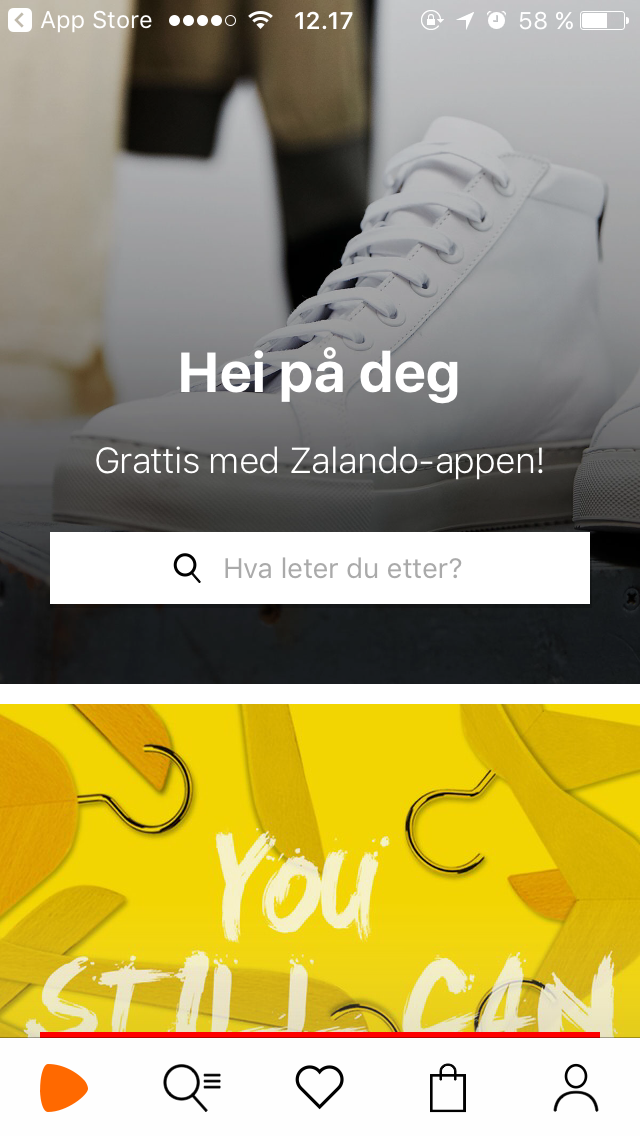
\includegraphics[scale=0.2]{images/inspiration/zalando1}
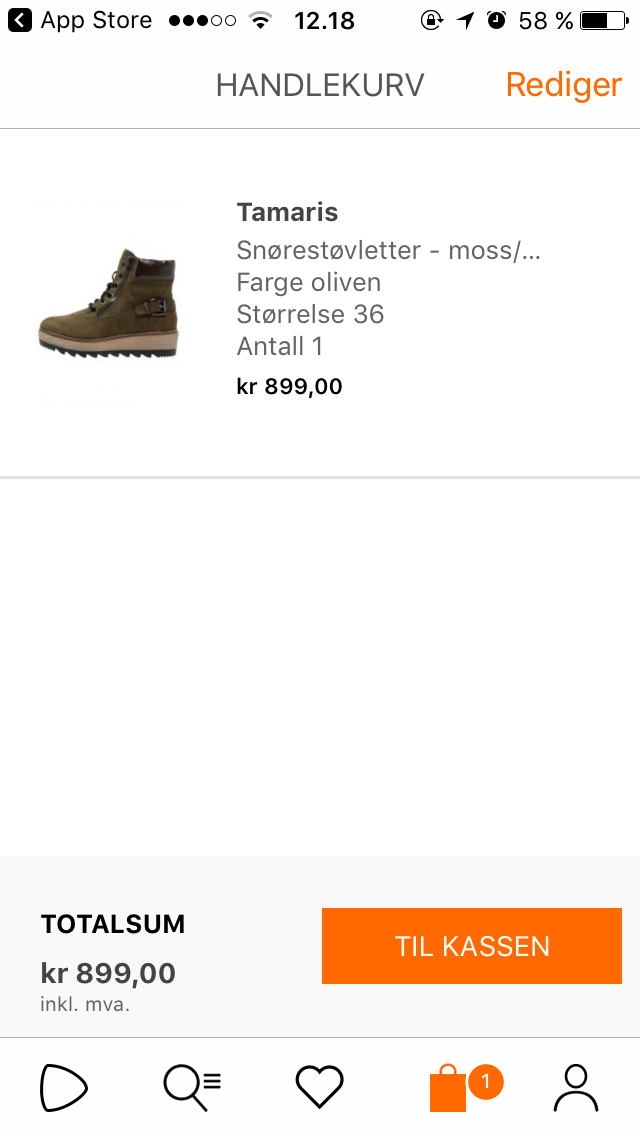
\includegraphics[scale=0.2]{images/inspiration/zalando2}
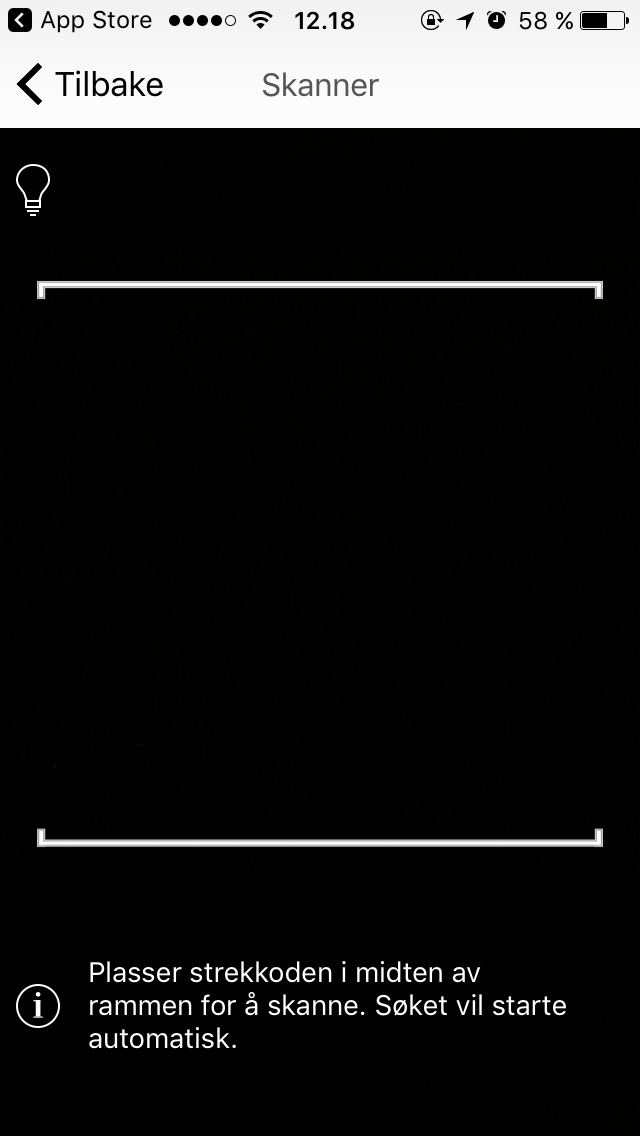
\includegraphics[scale=0.2]{images/inspiration/zalando3}
\centering %centering the image
\caption{Zalando}
\label{fig:Zalando}
\end{figure}

\subsection{Teknologiundersøkelse}
\label{teknologiundersokelse}
Også QR-koder og beacons er spesifisert som teknologi for prosjektet. QR-koder er kvadratiske bilder satt sammen av små firkanter som kan scannes med mobilkamera og sende brukeren videre til en nettside eller tekstfil\cite{prosjektoppgaven}. Dette ligner mye på strekkodene man finner på varer man handler i butikken. Beacons er derimot små Bluetooth-sendere som kontinuerlig sender ut små datapakker til omgivelsene sine med informasjon om sin ID og en tekst eller link til nettside\cite{prosjektoppgaven}. Bruken er den samme som ved QR-kode, men med beacons behøver ikke brukeren å scanne koden aktivt selv.
\\\\
RFID er kort for \textit{radio frequency identificator}, og er små merkelapper som kan festes på produktenes merkelapper\cite{rfid}. RFID-merkelapper er intelligente strekkoder som kan snakke med et nettverk, og med det kan kunden ha full oversikt over hva som er lagt i handlevognen. Merkelappene kommuniserer med en elektronisk leser som håndterer informasjonen. Dette er teknologi som også brukes til å lokalisere kjæledyr, biler og postforsendelser. Denne teknologien fant gruppen interessant, og ønsket å bruke den i videre arbeid.

 
 


